\section{Introduction}
\label{section:Introduction}

Given permutations $\pi$ and $\sigma_1, \sigma_2, \ldots, \sigma_k$,
the permutation $\pi$ is said to be
\emph{$(\sigma_1, \sigma_2, \ldots, \sigma_k)$-colorable},
denoted $\pi \in \sigma_1 \bullet \sigma_2 \bullet \dots \bullet \sigma_k$,
if there exists a $k$-coloring of $\pi$ (\emph{i.e.}, assign one color
among $k$ available colors to each element of $\pi$) such that the
pattern induced by each color $i$, $1 \leq i \leq k$, is order-isomorphic
to $\sigma_i$.
For example, $\pi = 192854367$ is $(12, 312, 4213)$-colorable
(\emph{i.e.}, $\pi \in 12 \bullet 312 \bullet 4213$) since
the patterns $15$, $926$ and $8537$ are order-isomorphic to
$12$, $312$ and $4213$, respectivelly.

The \textsc{$k$-Permutation Coloring} problem is defined as follows:
Given permutations $\pi$ and $\sigma_i$, $1 \leq i \leq k$, with
$|\pi| = \sum_{i=1}^k |\sigma_i|$,
decide the question
$\pi \in \sigma_1 \bullet \sigma_2 \bullet \dots \bullet \sigma_k$.

\begin{figure}
  \centering
  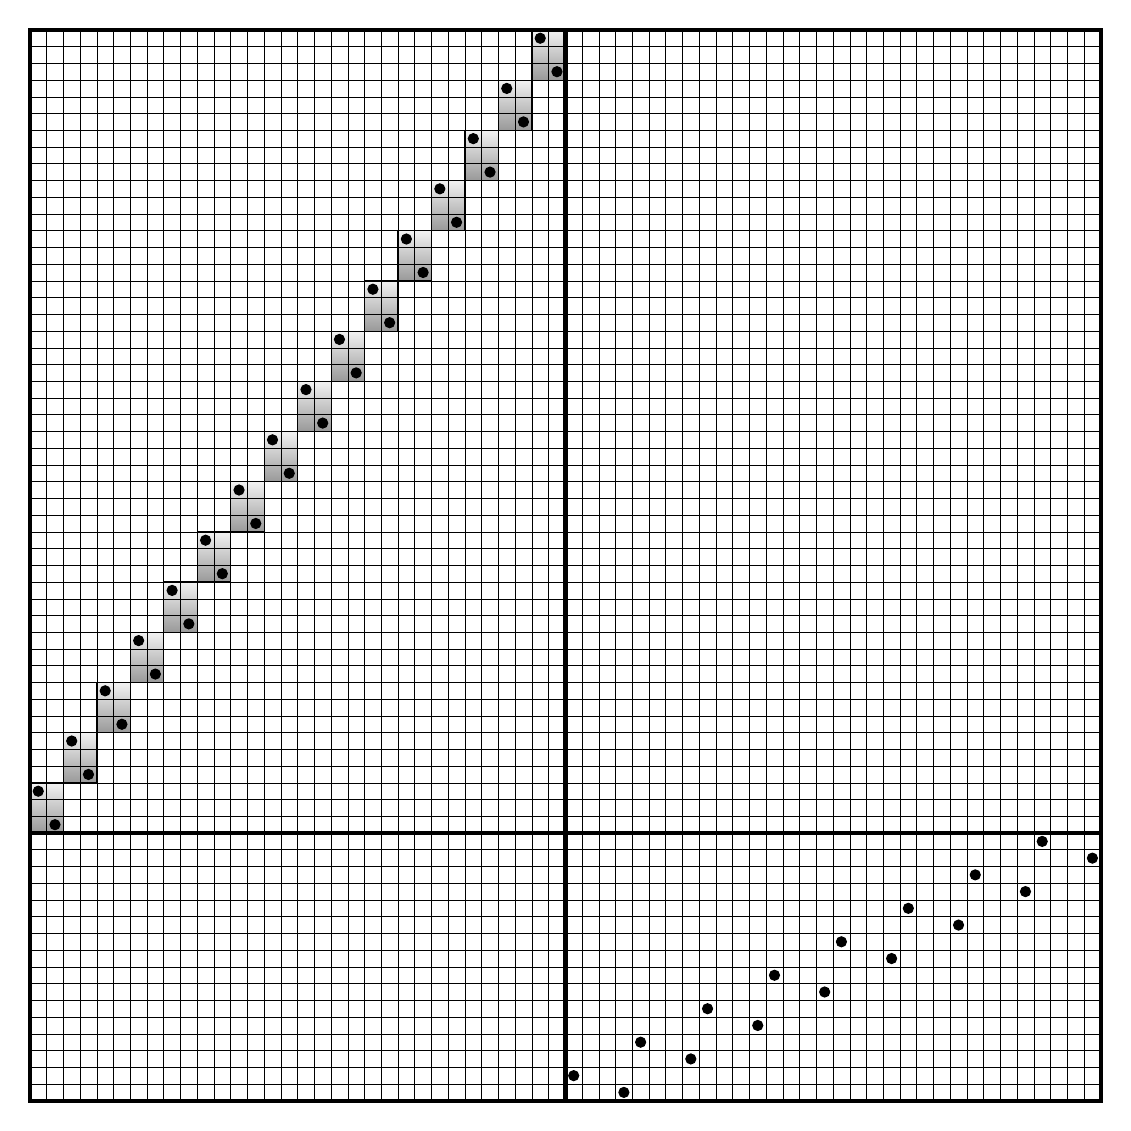
\begin{tikzpicture}
  [
    scale=.425,
    box/.style={
      shade,
      %blur shadow={shadow blur steps=5,shadow blur extra rounding=1.3pt},
      top color=black!5,
      bottom color=black!40
    },
    gadget/.style={
      box,
      rounded corners
    },
    r/.style={
      box,
      draw,
      ultra thick,
    }
  ]

  % vertices
  \foreach \v in {1,2,...,16} {
    \draw [box] (\v - 1, 7 + 1.5*\v - .5) rectangle (\v, 7 + 1.5*\v + 1);
    \draw [very thin,step=0.5cm] (\v - 1, 7 + 1.5*\v - .5) grid (\v, 7 + 1.5*\v + 1);
    \draw [fill=black] (\v - 1 + .25, 7 + 1.5*\v + .75) circle (0.15);
    \draw [fill=black] (\v - .25, 7 + 1.5*\v - .25) circle (0.15);
  }

  % edges
  \foreach \e in {1,2,...,8} {
      %\draw [box] (16 + \e*2, -1 + \e) rectangle (16 + \e*2, \e);
      %\draw [very thin,step=0.5cm] (16 + \e*2, -1 + \e) grid (17 + \e*2, \e);
      \draw [fill=black] (14.25 + \e*2, -.25 + \e) circle (0.15);
      \draw [fill=black] (15.75 + \e*2, -.75 + \e) circle (0.15);
  }

  \draw [ultra thick] (0,0) rectangle (32,32);
  \draw [very thin,step=0.5cm] (0,0) grid (32,32);

  \draw [ultra thick] (0,8) -- (32,8);
  \draw [ultra thick] (16,0) -- (16,32);
  \end{tikzpicture}
\end{figure}

